\documentclass{ethpresentation}

\title{Building a 25 MHz NMR Spectrometer}
\date{\today}
\author{Maximilian Stabel}
\institute{ETH Zürich}

\begin{document}
\maketitle

\section{Why?}

\begin{frame}{Accessing NMR in the South is hard}
  \centering
  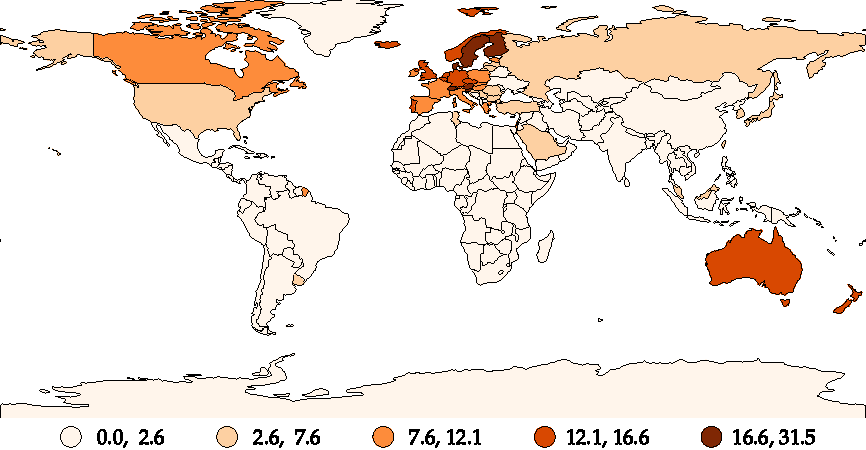
\includegraphics[height=0.8\textheight]{images/nmr-affiliations-per-million-people_naturalbreaks.pdf}

  \(\frac{\text{NMR affiliations}}{\text{million people}}\)
\end{frame}


\section{What already works}

\begin{frame}{We can already see water}
  \centering
  \includegraphics<1>[width=0.9\textwidth]{images/fid_sine_fit.pdf}
  \includegraphics<2>[width=0.9\textwidth]{images/fft_fit.pdf}
\end{frame}

\begin{frame}{We can even see Toluene peaks!}
  \centering
  \includegraphics<1>[width=0.9\textwidth]{images/fid_toluene.pdf}
  \includegraphics<2>[width=0.9\textwidth]{images/fft_toluene.pdf}
\end{frame}

\begin{frame}{Thank you!}
  \begin{columns}
    \begin{column}{0.5\textwidth}
      \centering
      \includesvg[width=0.5\textwidth]{./images/logo_magnETHical.svg}
    \end{column}
    \begin{column}{0.5\textwidth}
      \centering
      Find everything on \\ \vspace*{\baselineskip}

      \includesvg[width=0.5\textwidth]{./images/gitlab_qrcode.svg}

      \url{https://gitlab.ethz.ch/mstabel/nmr-spectrometer}
    \end{column}
  \end{columns}
\end{frame}

\appendix

\begin{frame}[standout]
  A backup graph for explaining things.
\end{frame}

\end{document}